\documentclass[9pt]{beamer}
\usepackage[utf8]{inputenc}
\usepackage[T1]{fontenc}
\usepackage{lmodern}
\usetheme{Dresden}

\usepackage{unicode-math}
\usepackage{circuitikz}

\setmathfont{Latin Modern Math}

\usepackage{graphicx}
\usepackage[spanish]{babel}

\usepackage{enumitem}

\usepackage{tikz}
\usetikzlibrary{%
	decorations.pathreplacing,%
	decorations.pathmorphing,
	decorations.markings%
}
\usetikzlibrary{patterns,calc,arrows}
\usepackage{pgfplots}
\definecolor{copper}{rgb}{1,1,0}
\definecolor{pcb}{rgb}{0,1,0}
% shades of them for the different elements
\colorlet{groundplane}{copper!50!black}
\colorlet{pcbfront}{pcb!50!black}
\colorlet{pcbright}{pcb!20!black}
\colorlet{pcbtopleft}{pcb!70!black}
\colorlet{pcbtopright}{pcb!50!black}
\colorlet{striplinefront}{copper!50!black}
\colorlet{striplineright}{copper!50!black}
\colorlet{striplinetopleft}{copper!90!black}
\colorlet{striplinetopright}{copper!60!black}
\pgfplotsset{compat=1.18}

\begin{document}
	\author{Recalde Santiago; Villar Federico Ignacio}
	\title{Amplificador de Microondas}
	\subtitle{Trabajo Práctico 2}
	%\logo{}
	\institute{FCEFyN UNC}
	%\date{}
	\subject{Electrónica Analógica III}
	%\setbeamercovered{transparent}
	%\setbeamertemplate{navigation symbols}{}
	
	\pgfarrowsdeclarecombine{dimarrow}{dimarrow}{latex}{latex}{}{}
	\def\Dimline[#1][#2][#3]{
		\draw[ % |-|, % removed, looks odd for l
		decoration={markings, % switch on markings
			mark=at position 0 with {\arrowreversed[scale=0.5]{dimarrow}};,
			mark=at position .5 with {\node[black] at (0,0.25) {#3};},
			mark=at position 1 with {\arrow[scale=0.5]{dimarrow}};,
		},
		postaction=decorate] #1 -- #2 ;
	}
	
	
	\begin{frame}[plain]
		\maketitle
	\end{frame}
	
	\section{Introducción}
	\begin{frame}
		\frametitle{Enunciado (I)}
		
		Diseñar, Simular e implementar un amplificador de microondas de baja señal para máxima ganancia (adaptación conjugada simultánea). Utilizar cualquier método de adaptación de impedancias. Diseñar los acoplamientos utilizando microstrips sobre un material FR4. La impedancia característica del sistema, impedancia de fuente e impedancia de carga son todas $50 \ \Omega$. Utilizar:
		\begin{itemize}
			\item Transistor \textbf{BFP450}
			\item Frecuencia $1.8 \ GHz$
		\end{itemize}
		Realizar el diseño, simulación, PCB e informe técnico. Entregar el archivo del informe en PDF y el archivo del proyecto.
	\end{frame}
	
	\begin{frame}{Enunciado (II)}
		El trabajo debe incluir:
		\begin{itemize}
			\item Selección del punto de reposo del dispositivo.
			\item Análisis de estabilidad.
			\item Cálculo de coeficientes de reflexión e impedancias de entrada y salida.
			\item Diseño de los acoplamientos de entrada y salida.
			\item Cálculo de polarización.
			\item Circuito esquemático completo.
			\item Simulación en software de desarrollo para alta frecuencia mostrando los coeficientes de reflexión de entrada, salida, ganancia directa e inversa del amplificador completo.
			\item Diseño del PCB para el amplificador completo.
			\item Medición efectuada.
		\end{itemize}
	\end{frame}
	
	\begin{frame}{Low Noise Amplifier (I)}
		Las antenas se rigen por el principio de reciprocidad, esto significa que las características de transmisión y recepción de una antena son idénticas. No tienen diferencias en atributos como la ganancia de transmisión de recepción, el ancho del haz o los patrones de radiación entre los dos modos. 
		
		La reciprocidad es un principio de diseño simplificador, pero las rutas de los dos lados de transmisión y recepción son mucho más que solo la antena. El lado de transmisión tiene una tarea sencilla: tomar una señal conocida y relativamente fuerte con atributos definidos, que pasó por el amplificador de potencia y lo presenta a la antena. Ahora, en cuanto a la ruta del receptor, el caso es ligeramente más complicado, hay que localizar y capturar una pequeña cantidad de potencia de señal de RF y actuar como un transductor de campo electromagnético para convertir esa potencia en un voltaje utilizable. Necesita hacer esto a pesar del ruido en la banda y la interferencia de diversos tipos y fuentes, así como desviaciones del transmisor y cambios de frecuencia inducidos por el efecto Doppler (en algunas aplicaciones).
	\end{frame}	
		
	\begin{frame}{Low Noise Amplifier (II)}
		Esa potencia es baja, del orden de los milivatios o microvatios, y, por consecuencia, el voltaje inducido en la antena suele ser del orden de los microvoltios. La solución es amplificar la señal que se tiene entonces. 
		
		La señal a amplificar tiene ruido, y por consiguiente, la relación señal/ruido (\textbf{SNR}) afecta a la capacidad de demodular y decodificar la señal recibida. Una de las métricas importantes en comunicaciones digitales es el Bit Error Rate con respecto a la Signal to Noise Ratio. Los detalles de esas curvas dependen de muchos factores, incluida la intensidad de la señal recibida, la SNR y el tipo de codificación del código de corrección de errores (ECC) de los datos sin procesar que se utiliza en el transmisor.
		
		Resta ahora entender que la amplificación aumenta la magnitud de la señal, pero a la vez degrada la SNR, y, por lo tanto, el rendimiento del enlace también empeora. 
	\end{frame}
	
	\begin{frame}{Low Noise Amplifier (III)}
		El amplificador de bajo ruido (\textbf{LNA}) de front-end tiene dos características de interes principal:
		\begin{itemize}
			\item Agrega poco ruido a la señal
			\item Tiene alta ganancia
		\end{itemize}
		
		Otro tema crucial es dónde colocar físicamente el LNA. Colocarlo con el resto del circuito significa que el inevitable ruido térmico del cable que transporta la señal amplificada desde el LNA al sistema se agregará a la señal no amplificada, lo que reducirá aún más la SNR. Por esta razón, incluso las aplicaciones de consumo, como las antenas parabólicas de terminal de muy pequeña apertura (VSAT), colocan el LNA justo en el punto focal de la antena.
	\end{frame}	
	
	\begin{frame}{Low Noise Amplifier (IV)}
		El diagrama en bloques de la conexión front-end a la que se hace referencia, y que tiene como objetivo ser resuelta por este trabajo práctico es el siguiente.

		\begin{figure}
			\centering
			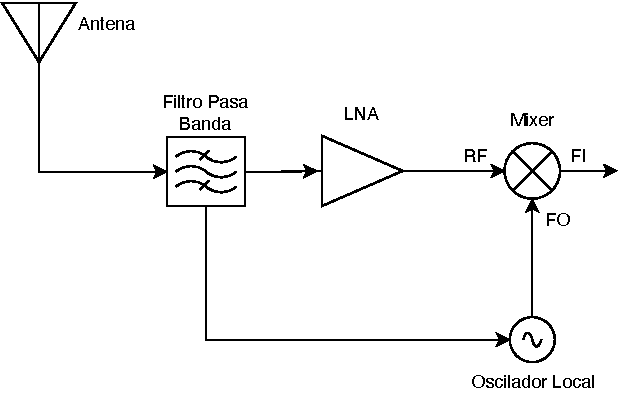
\includegraphics[width=0.7\linewidth]{img/lna_front}
			\caption{Ubicación amplificador LNA.}
			\label{fig:lnafront}
		\end{figure}		
	\end{frame}
	
	\begin{frame}{Parámetros S (I)}
		
		Los parámetros S describen la respuesta de una red de N puertos a señales incidentes en cualquiera o en todos los puertos. El primer número en el subíndice se refiere al puerto que responde, mientras que el segundo número se refiere al puerto incidente. Así, S21 significa la respuesta en el puerto 2 debido a una señal en el puerto 1. Las redes de N puertos más comunes en microondas son redes de uno y dos puertos.
		
		\begin{figure}
			\centering
			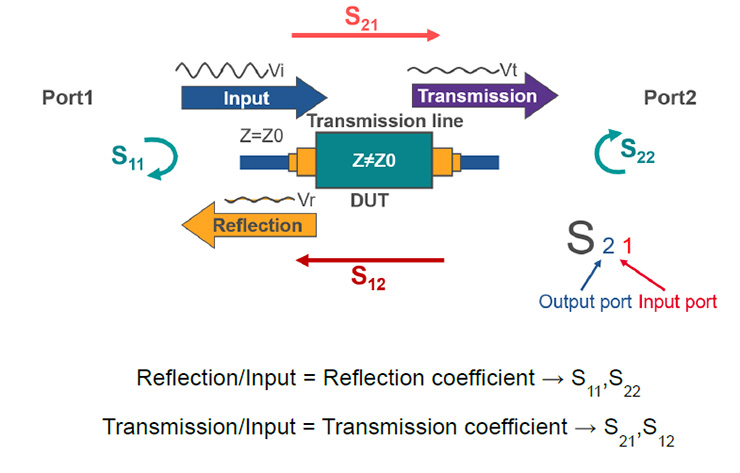
\includegraphics[width=0.5\linewidth]{img/s_params_img}
			\caption {Parámetros S para una línea de transmisión de dos puertos.}
			\label{fig:sparamsimg}
		\end{figure}
		
	\end{frame}
	
	\begin{frame}{Parámetros S (II)}
		Puede redibujarse de la siguiente manera lo planteado en la filmina anterior.
		\begin{figure}
			\centering
			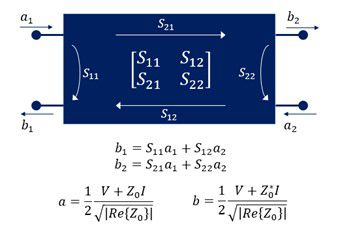
\includegraphics[width=0.6\linewidth]{img/s_block}
			\caption{Red de dos puertos con parámetros de dispersión.}
			\label{fig:sblock}
		\end{figure}
		
	\end{frame}
	
	\begin{frame}{Líneas de transmisión}
		Una línea de transmisión es una estructura material de geometría uniforme utilizada para transportar eficientemente la energía de radiofrecuencia desde un punto a otro; como puede ser de un equipo de transmisión a otro, de un transmisor a la antena, entre otras aplicaciones. Un parámetro que la define comúnmente es su impedancia característica.
		
		La denominación de línea de transmisión se usa exclusivamente para aquellos medios de transmisión con soporte físico, susceptibles de guiar ondas electromagnéticas en modo \textbf{TEM} (modo transversal electromagnético). Un modo TEM se caracteriza por el hecho de que tanto el campo eléctrico, como el campo magnético que forman la onda son perpendiculares a la dirección en que se propaga la energía; sin existir, por tanto componente de los campos en la dirección axial (dirección en que se propaga la energía).
	\end{frame}
	
	\begin{frame}{Microstrip (I)}
		Un microstrip es un tipo de línea de transmisión eléctrica que puede ser fabricada utilizando placa de circuito impreso (PCB). Se utiliza para transmitir señales de microondas.
		
		Construida en una tarjeta de circuitos impresos, con 2 conductores, uno en un lado de la tarjeta y el otro el plano de Tierra. Se utilizan en sistemas de microondas.
		
		Consiste en una franja de conducción separada de la franja de masa por una capa de sustrato dieléctrico. Componentes de microondas, tales como antenas, acopladores, filtros, divisores, etc. pueden formarse a partir de microstrip, haciendo dicho componente como una metalización sobre el sustrato. El microstrip hasta ahora es más barato que la tecnología tradicional de guía de onda, además de ser mucho más ligero y compacto.
	\end{frame}
	
	\begin{frame}{Microstrip (II)}
		Para el análisis y síntesis de microtiras, en el trabajo práctico se trabaja con el modelo empírico de Hammerstad. Las variables de interés en el circuito físico son las siguientes:
		
		\begin{itemize}
			\item Espesor del dieléctrico: $h$
			\item Espesor del conductor: $t$
			\item Ancho de la pista: $w$
			\item Longitud de la pista: $l$
			\item Permitividad del dieléctrico: $\epsilon$
		\end{itemize}
		
	\end{frame}
	
	\begin{frame}{Microstrip (III)}
		El modelo gráfico que tiene las variables mencionadas anteriormente es el siguiente:
		
		\begin{center}
			\begin{figure}
			
			\begin{tikzpicture}
				% PCB back, not visible, so it can be skiped
				%\filldraw [white](0,0,0) -- (0,1,0) -- (5,1,0) -- (5,0,0) -- (0,0,0);
				
				% PCB front, use cycle to close path
				\filldraw [pcbfront] (0,0,5) coordinate (height bottom) -- (0,1,5) coordinate (height top) -- (5,1,5) -- (5,0,5) -- cycle;
				
				% PCB top
				\shade[top color = pcbtopleft, bottom color = pcbtopright, shading angle=75] (0,1,0) -- (5,1,0) -- (5,1,5) -- (0,1,5) -- cycle;
				
				% PCB right, closed it
				\filldraw [pcbright] (5,0,0) -- (5,0,5) -- (5,1,5) -- (5,1,0) -- cycle;
				
				% groundplane
				\filldraw [groundplane] (0,0,5) -- (5,0,5) -- (5,0,0) -- (5,-0.2,0) -- (5,-0.2,5) -- (0,-0.2,5) -- cycle;
				
				% stripline front
				\filldraw [striplinefront] (1.5,1.2,5) coordinate (length front) -- (3.5,1.2,5) coordinate (thickness top) -- (3.5,1,5) coordinate (thickness bottom) -- (1.5,1,5) -- cycle;
				
				% stripline front, duplicate
				%\filldraw [lightgray] (1.5,1.2,5) -- (3.5,1.2,5) -- (3.5,1,5) -- (1.5,1,5) -- cycle;
				
				%stripline top
				\shade [top color = striplinetopleft, bottom color = striplinetopright, shading angle=75] (1.5,1.2,0) coordinate (width left) coordinate (length back) -- (3.5,1.2,0) coordinate (width right)  -- (3.5,1.2,5) -- (1.5,1.2,5) -- cycle;
				
				% stripline right
				\filldraw [striplineright] (3.5,1,5) -- (3.5,1.2,5) -- (3.5,1.2,0) -- (3.5,1,0) -- cycle;
				
				\node at (4,0.5,5) {$\varepsilon$};
				
				% nodes no longer needed
				%\node at (1.5,1.5,0) (nA) {};
				%\node at (3.5,1.5,0) (nB) {};
				% stripline width
				\Dimline[($(width left)+(0,1,0)$)][($(width right)+(0,1,0)$)][$w$];
				\draw ($(width left)+(0,0.1,0)$) -- ($(width left)+(0,1.1,0)$);
				\draw ($(width right)+(0,0.1,0)$) -- ($(width right)+(0,1.1,0)$);
				
				% nodes no longer needed
				%\node at (-1.5,0.2,0) (nA) {};
				%\node at (-1.5,0.2,5) (nB) {};
				% stripline length
				\Dimline[($(length back)+(-2.5,0,0)$)][($(length front)+(-2.5,0,0)$)][$l$]; %[left];
				\draw ($(length front)+(-0.1,0,0)$) -- ($(length front)+(-2.6,0,0)$);
				\draw ($(length back)+(-0.1,0,0)$) -- ($(length back)+(-2.6,0,0)$); 
				
				% nodes no longer needed
				%\node at (7,0,5) (nA) {};
				%\node at (7,0.2,5) (nB) {};
				% stripline thickness
				\Dimline[($(thickness top)+(3.5,0,0)$)][($(thickness bottom)+(3.5,0,0)$)][$t$]; %[left];
				\draw ($(thickness top)+(0.1,0,0)$) -- ($(thickness top)+(3.6,0,0)$);
				\draw ($(thickness bottom)+(0.1,0,0)$) -- ($(thickness bottom)+(3.6,0,0)$);      
				
				% nodes no longer needed
				%\node at (-1.5,0,5) (nA) {};
				%\node at (-1.5,-1,5) (nB) {};
				% PCB height
				\Dimline[($(height top)+(-1,0,0)$)][($(height bottom)+(-1,0,0)$)][$h$]; %[left];   
				\draw ($(height top)+(-0.1,0,0)$) -- ($(height top)+(-1.1,0,0)$);
				\draw ($(height bottom)+(-0.1,0,0)$) -- ($(height bottom)+(-1.1,0,0)$);
				
			\end{tikzpicture}
			\caption{Modelo de referencia para las microstrips.}
		\end{figure}
		\end{center}
		
	\end{frame}
	
	\section{Diseño}
	
	\begin{frame}{Selección del punto de trabajo (I)}
		Para seleccionar el punto de trabajo del transistor BFP450, se ploteó un mapa de calor, en donde las coordenadas representan $V_{CE}$ e $I_C$, y el color muestra qué tan estable es la configuración. Mientras más verdoso es el color, la condición de incondicionalmente estable se cumple con mayor holgura. Para hacer este mapa se analizó mediante un script de Python cada una de las posibilidades de estabilidad incondicional. 
		
		Para verificar la estabilidad del sistema polarizado, se analizaron las siguientes variables:
		
		\begin{itemize}
			\item $k$
			\item $\Delta$
			\item $S_{11}$, $S_{12}$, $S_{21}$, $S_{22}$
			\item $\Lambda_{in}$, $\Lambda_{out}$
			\item $Z_{in}$, $Z_{out}$
			\item $Z_L$, $Z_S$
		\end{itemize}
	\end{frame}
	
	\begin{frame}{Selección del punto de trabajo (II)}
		El mapa de calor resultante es el siguiente:
		\begin{figure}
			\centering
			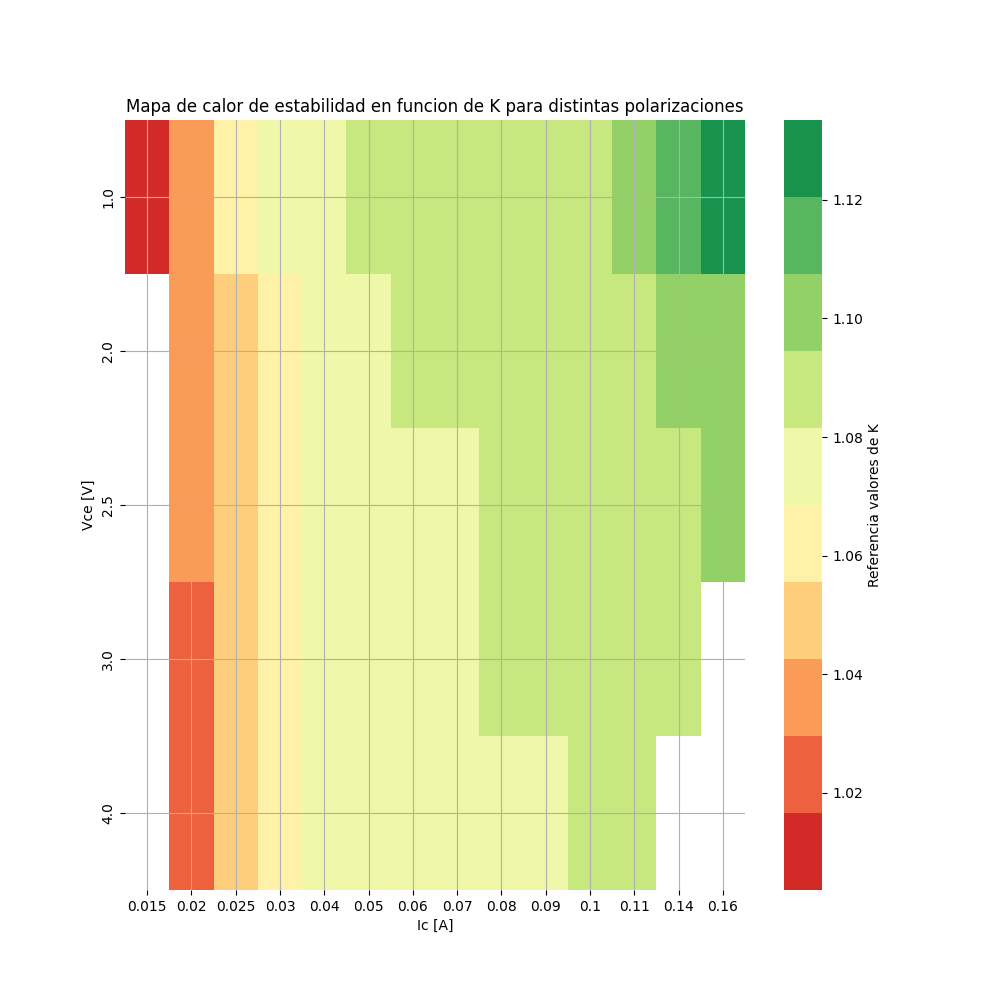
\includegraphics[width=1\linewidth]{../heatmap}
			\caption{Mapa de calor obtenido.}
			\label{fig:heatmap}
		\end{figure}
		
	\end{frame}
	
	\begin{frame}{Selección del punto de trabajo (III)}
		Se define el punto de operación como: $I_C=0.11 \ A$ y $V_{CE}=1 \ V$. Los parámetros de dispersión para esta polarización están representados en el siguiente diagrama de Bode.
		\begin{figure}
			\centering
			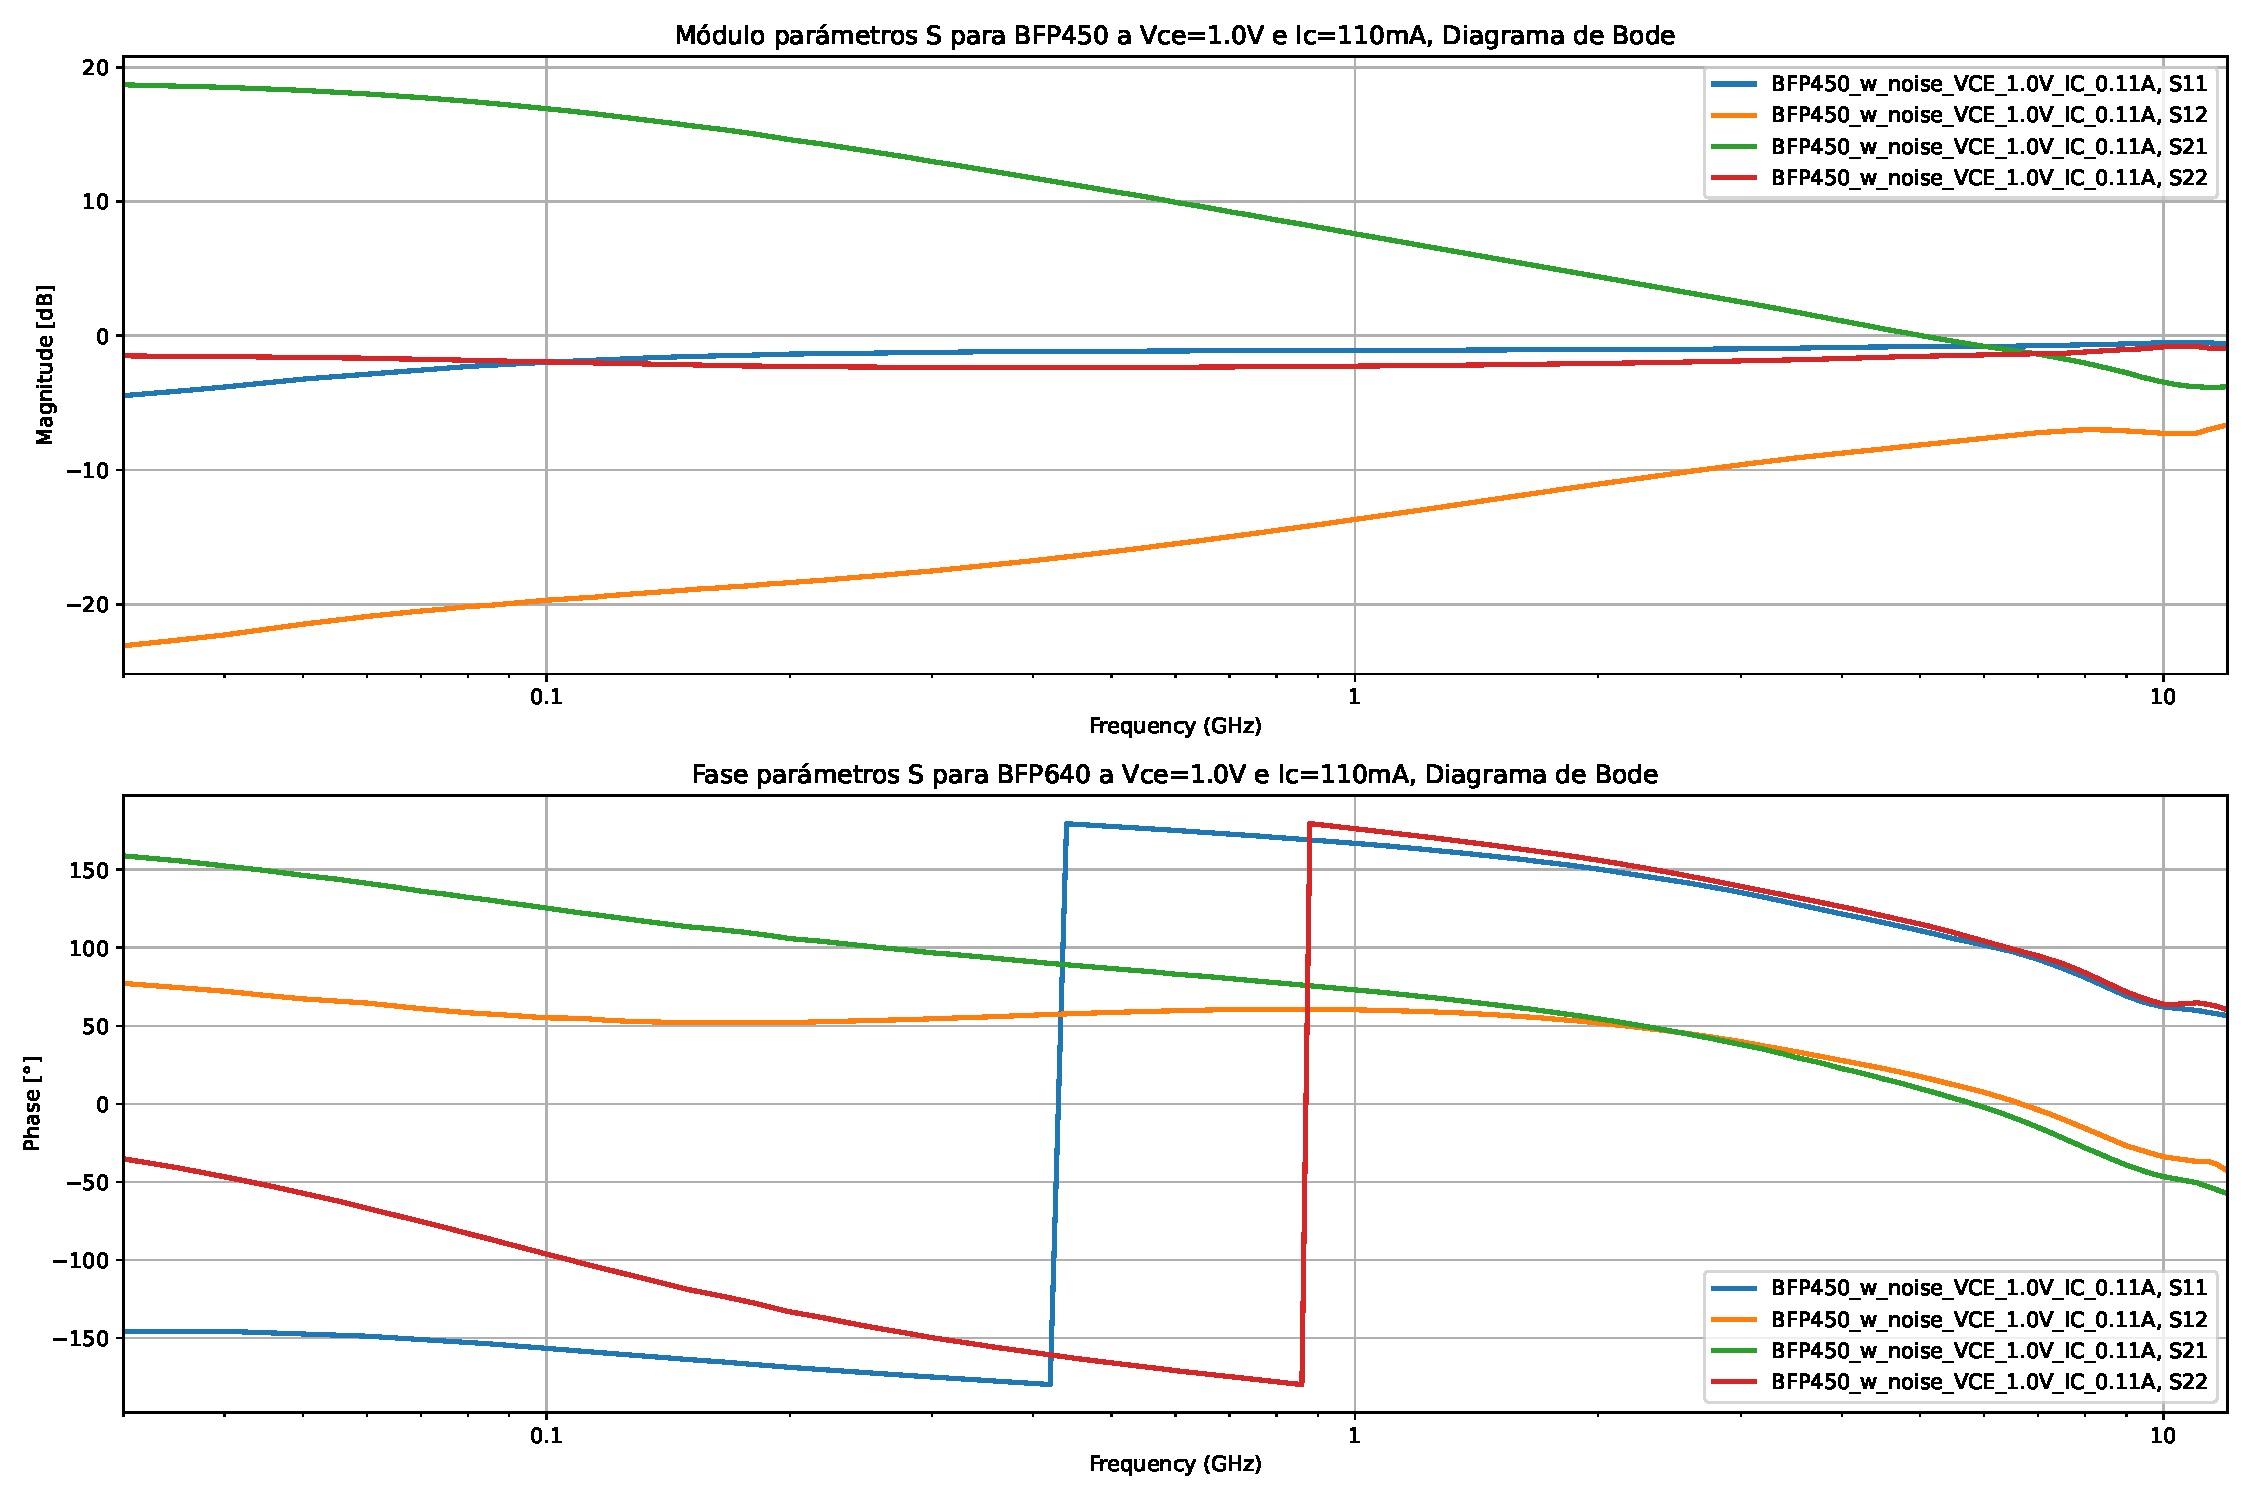
\includegraphics[width=0.7\linewidth]{../bfp450_vce_1_ic_0.11}
			\caption{Parámetros de dispersión para polarización seleccionada.}
			\label{fig:bfp450vce1ic0}
		\end{figure}
	\end{frame}
	
	\begin{frame}{Cálculo de la polarización (I)}
		Para la polarización, se decide utilizar una inyección de base, con ciertas variaciones, mostrada en la figura de a continuación.
		
		\begin{figure}
			\centering
			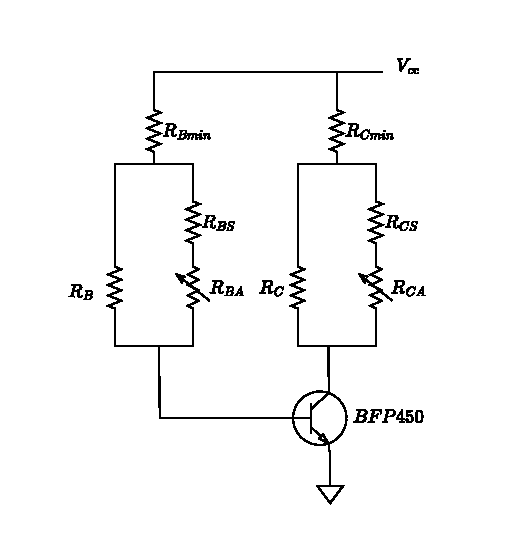
\includegraphics[width=0.5\linewidth]{img/polarizacion}
			\caption{Polarización utilizada.}
			\label{fig:polarizacion}
		\end{figure}
		
	\end{frame}
	
	\begin{frame}{Cálculo de la polarización (II)}
		Las resistencias mínimas:
		\begin{itemize}[label=\textbullet]
			\item $R_{Bmin}$
			\item $R_{Cmin}$
		\end{itemize}
		Permiten que nunca se superen las corrientes máximas de base y colector, para de esa forma evitar daños.
		
		La alimentación $V_{CC}$ está planteada en $4 \ V$, de modo que un eventual estado de corte en el transistor no permita que la $V_{CE}$ no sobrepase el máximo de ruptura.
		
		$$ I_{Cmax}=\frac{V_{CC}}{R_{Cmin}}=\frac{4 \ V}{25 \ \Omega}=160 \ mA$$
		
		$$ I_{Bmax}=\frac{V_{CC}-V_{BE}}{R_{Bmin}} = \frac{4 \ V - 0.9 \ V}{2 \ k\Omega}=1.55 \ mA$$
	\end{frame}
	
	\begin{frame}{Cálculo de la polarización (III)}
		$$ R_{CT} = \frac{V_{CC}-V_{CE}}{I_C} = \frac{4 \ V - 1 \ V}{110 \ mA}=27.27 \ \Omega$$
		$$ R_{BT} = \frac{V_{CC}-V_{BE}}{I_B} = \frac{4 \ V - 0.9 \ V}{1.375 \ mA}=2255 \ \Omega$$
		
		Finalmente:
		\begin{itemize}[label=\textbullet]
			\item $R_{Bmin} = 2 \ k\Omega$
			\item $R_{BS} = 300 \Omega$
			\item $R_B = 1 \ k\Omega$
			\item $R_{BA} = 100 \Omega$
			\item $R_{Cm} = 1 \ \Omega$
			\item $R_{CS} = 120 \Omega$
			\item $R_C= 32 \ \Omega$
			\item $R_{CA} = 100 \Omega$
		\end{itemize}
	\end{frame}
	
	\begin{frame}{Alimentación del circuito}
		Para alimentar el circuito, se trabajó con un regulador LM317, en una confguración de fuente de tensión continua variable. Se busca con esto eliminar el riple de la fuente de alimentación y proveer una tensión constante. Se utilizó la topología siguiente:
		
		\begin{figure}
			\centering
			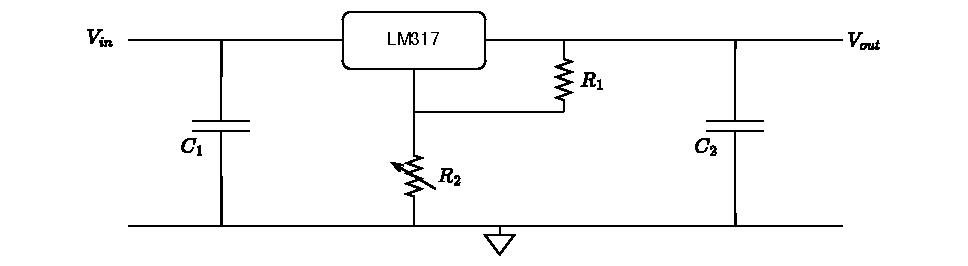
\includegraphics[width=0.5\linewidth]{img/lm317}
			\caption{Circuito de alimentación utilizado.}
			\label{fig:lm317}
		\end{figure}
		
		En donde: 
		
		\begin{itemize}[label=\textbullet]
			\item $C_1 = 0.1 \ \mu F$
			\item $C_2 = 47 \ \mu F$
		    \item $R_1 = 200 \ \Omega$
			\item $R_2 = 10 \ k \Omega$
		\end{itemize}
		
	\end{frame}
	
	\begin{frame}{Diseño de las líneas de transmisión (I)}
		En cuanto a las líneas de transmisión, para su diseño se empleó un script de Python, que permitió calcular los diferentes parámetros para las microstrips,  en este caso, esos parámetros son:
		
		\begin{itemize}[label=\textbullet]
			\item $w$
			\item $Z_0$
			\item $L$
			\item $\epsilon_{ef}$
			\item $w_{ef}$
		\end{itemize}
		
		Para simplificar los cálculos, se implementó un script de Python que tiene las operaciones del modelo empírico de Hammerstad, para de esa forma simplemente trabajar con las funciones, pasando como parámetros las diferentes características del material con el que se trabajó y los requerimientos.
		
	\end{frame}
	
	\begin{frame}{Diseño de las líneas de transmisión (II)}
		De los cálculos mencionados antes, se obtiene un circuito como el que se muestra a continuación.
		
		\begin{figure}
			\centering
			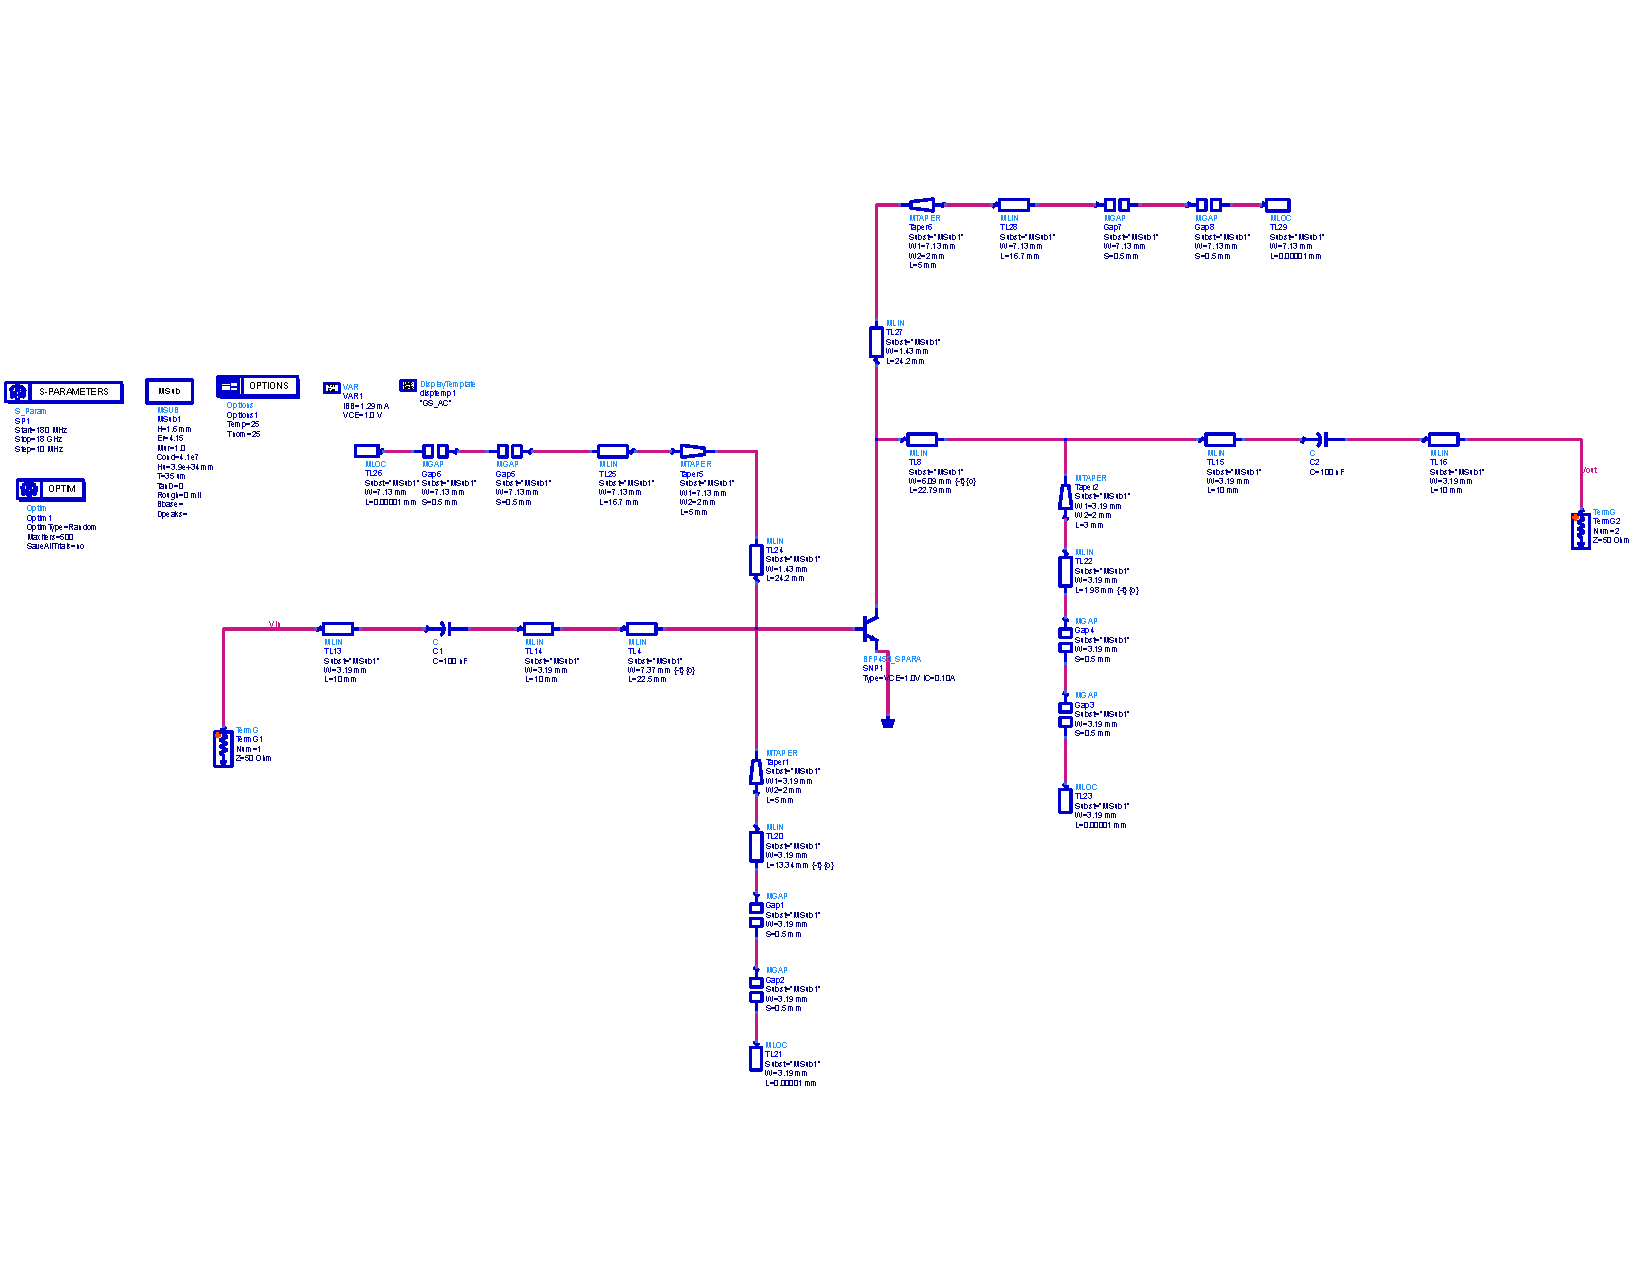
\includegraphics[width=0.8\linewidth]{img/sch_ads}
			\label{fig:schads}
			\caption{Esquemático obtenido.}
		\end{figure}
		
	\end{frame}
	
	\begin{frame}{Diseño de las líneas de transmisión (III)}
		Para las microstrips de $50 \ \Omega$, se tiene:
		\begin{figure}
			\centering
			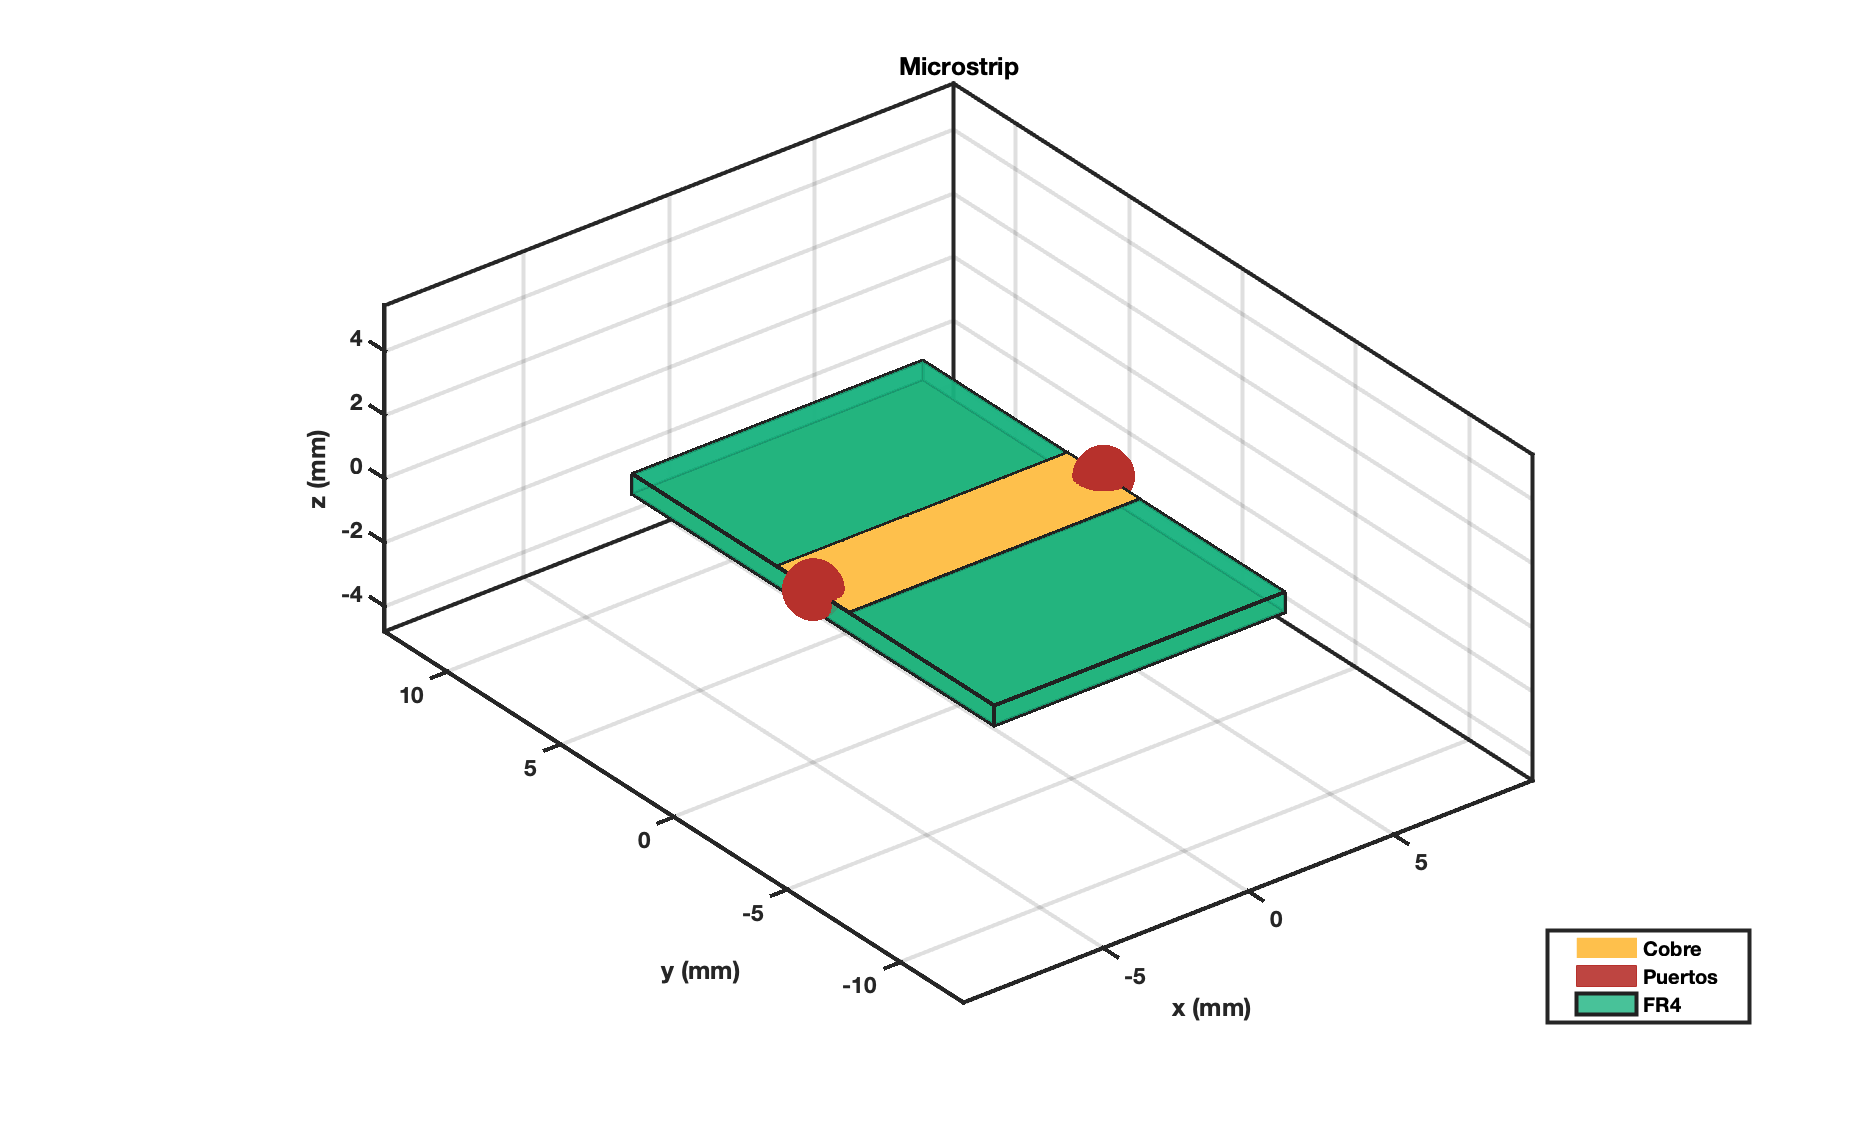
\includegraphics[width=0.8\linewidth]{../microstrip_p}
			\caption{DIseño de microstrip de $Z_0=50 \ \Omega$.}
			\label{fig:microstripp}
		\end{figure}
	
	\end{frame}
	
	\begin{frame}{Diseño de las líneas de transmisión (IV)}
		Para la etapa de entrada del amplificador, en donde se tiene un transformador de $\lambda /4$ y un stub diseñado para actuar como capacitor, se tiene.
		
		\begin{figure}
			\centering
			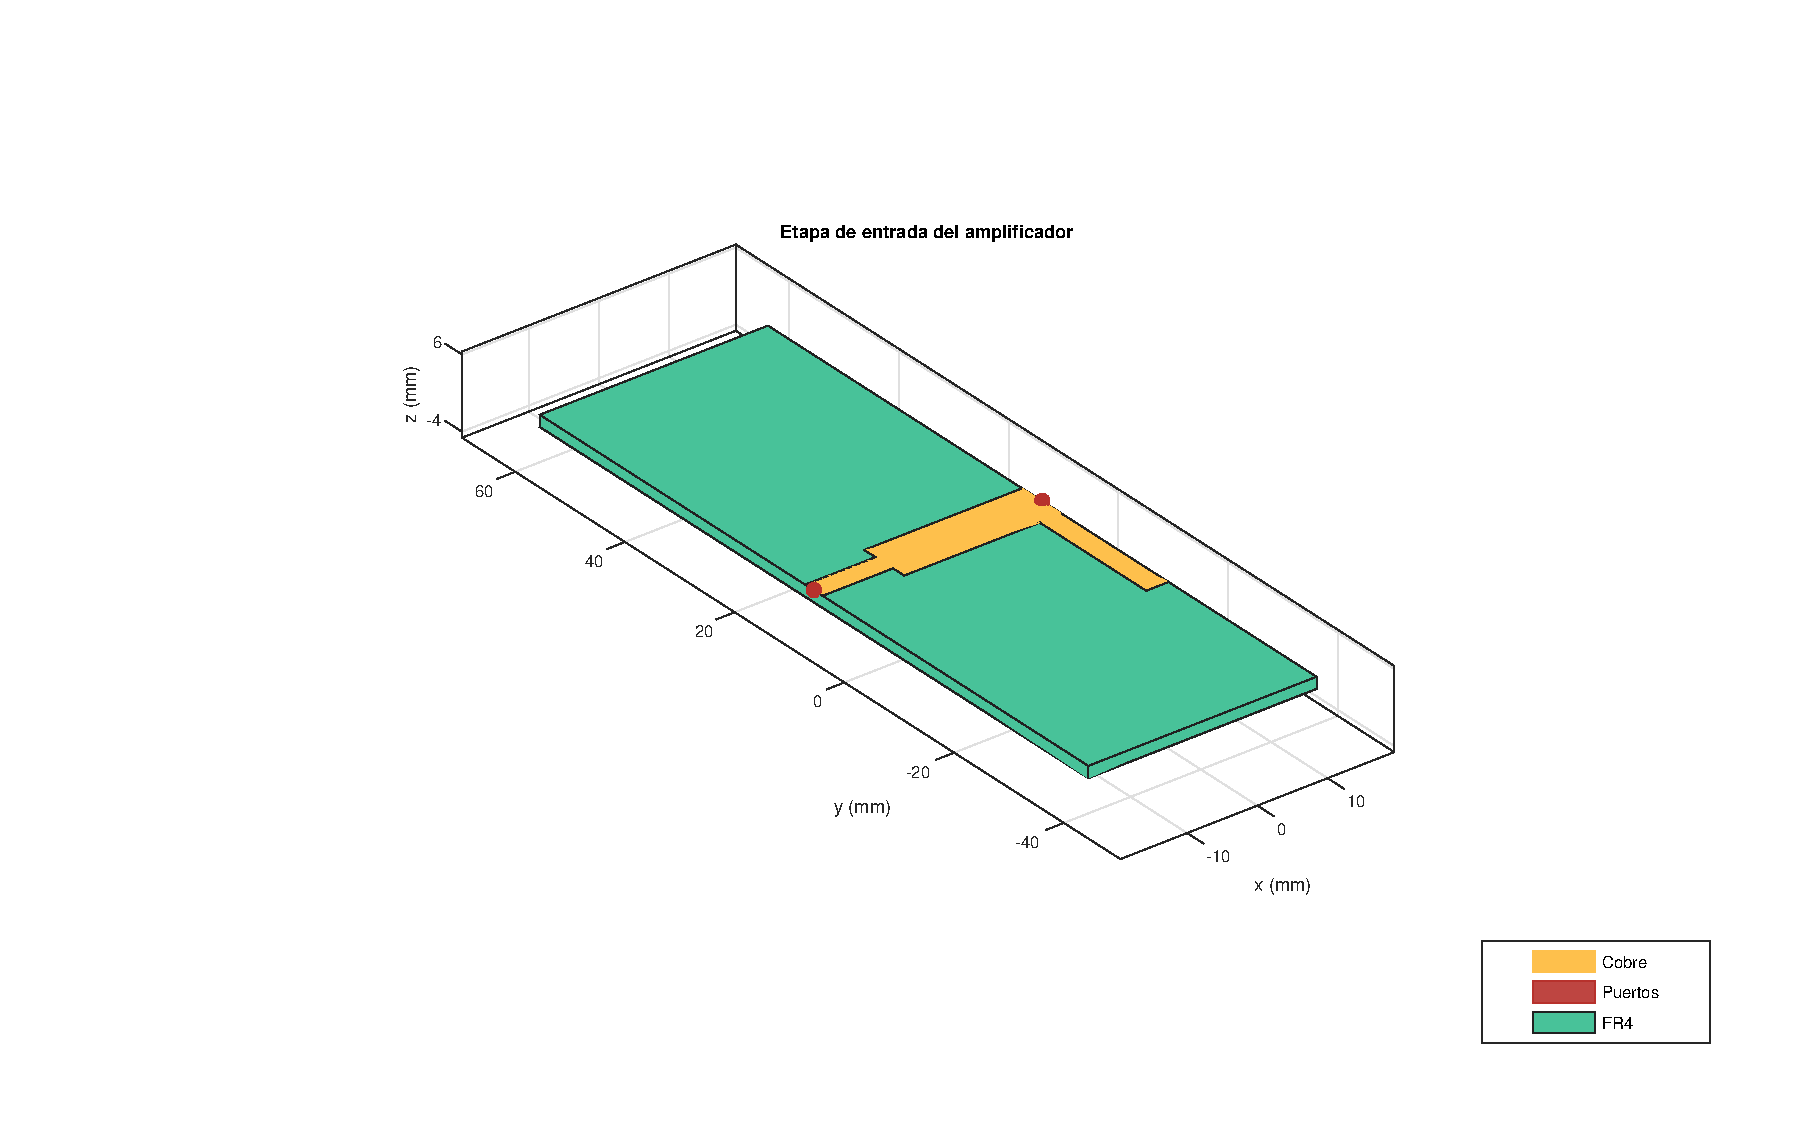
\includegraphics[width=0.8\linewidth]{../entrada}
			\caption{Diseño etapa de entrada.}
			\label{fig:entrada}
		\end{figure}
		
	\end{frame}
	
	\begin{frame}{Diseño de las líneas de transmisión (V)}
		Ahora, para la etapa de salida del amplificador, en donde se tiene un transformador de $\lambda /4$ y un stub diseñado para actuar como capacitor, se tiene.
		
		\begin{figure}
			\centering
			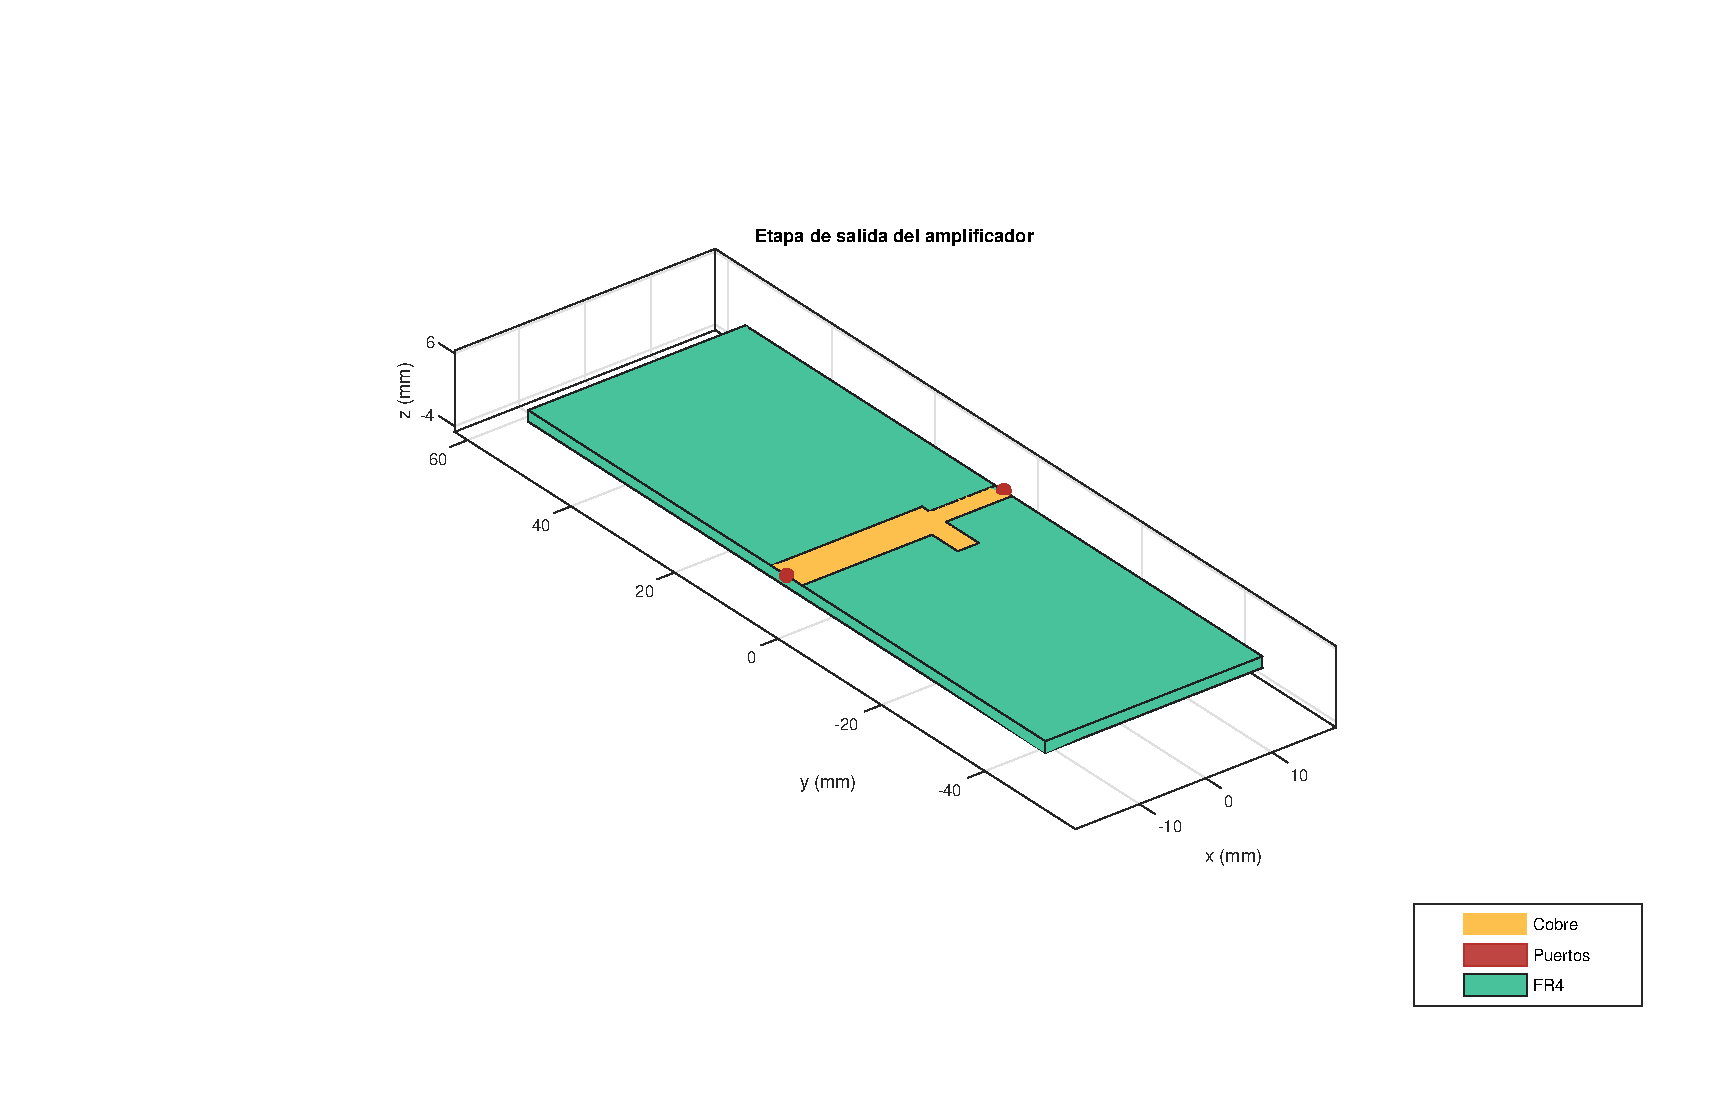
\includegraphics[width=0.8\linewidth]{../salida}
			\caption{Diseño etapa de salida.}
			\label{fig:salida}
		\end{figure}
		
	\end{frame}
	
	\begin{frame}{Diseño de las líneas de transmisión (VI)}
		Finalmente, el layout implementado, diseñado en inkscape, es el siguiente:
		\begin{figure}
			\centering
			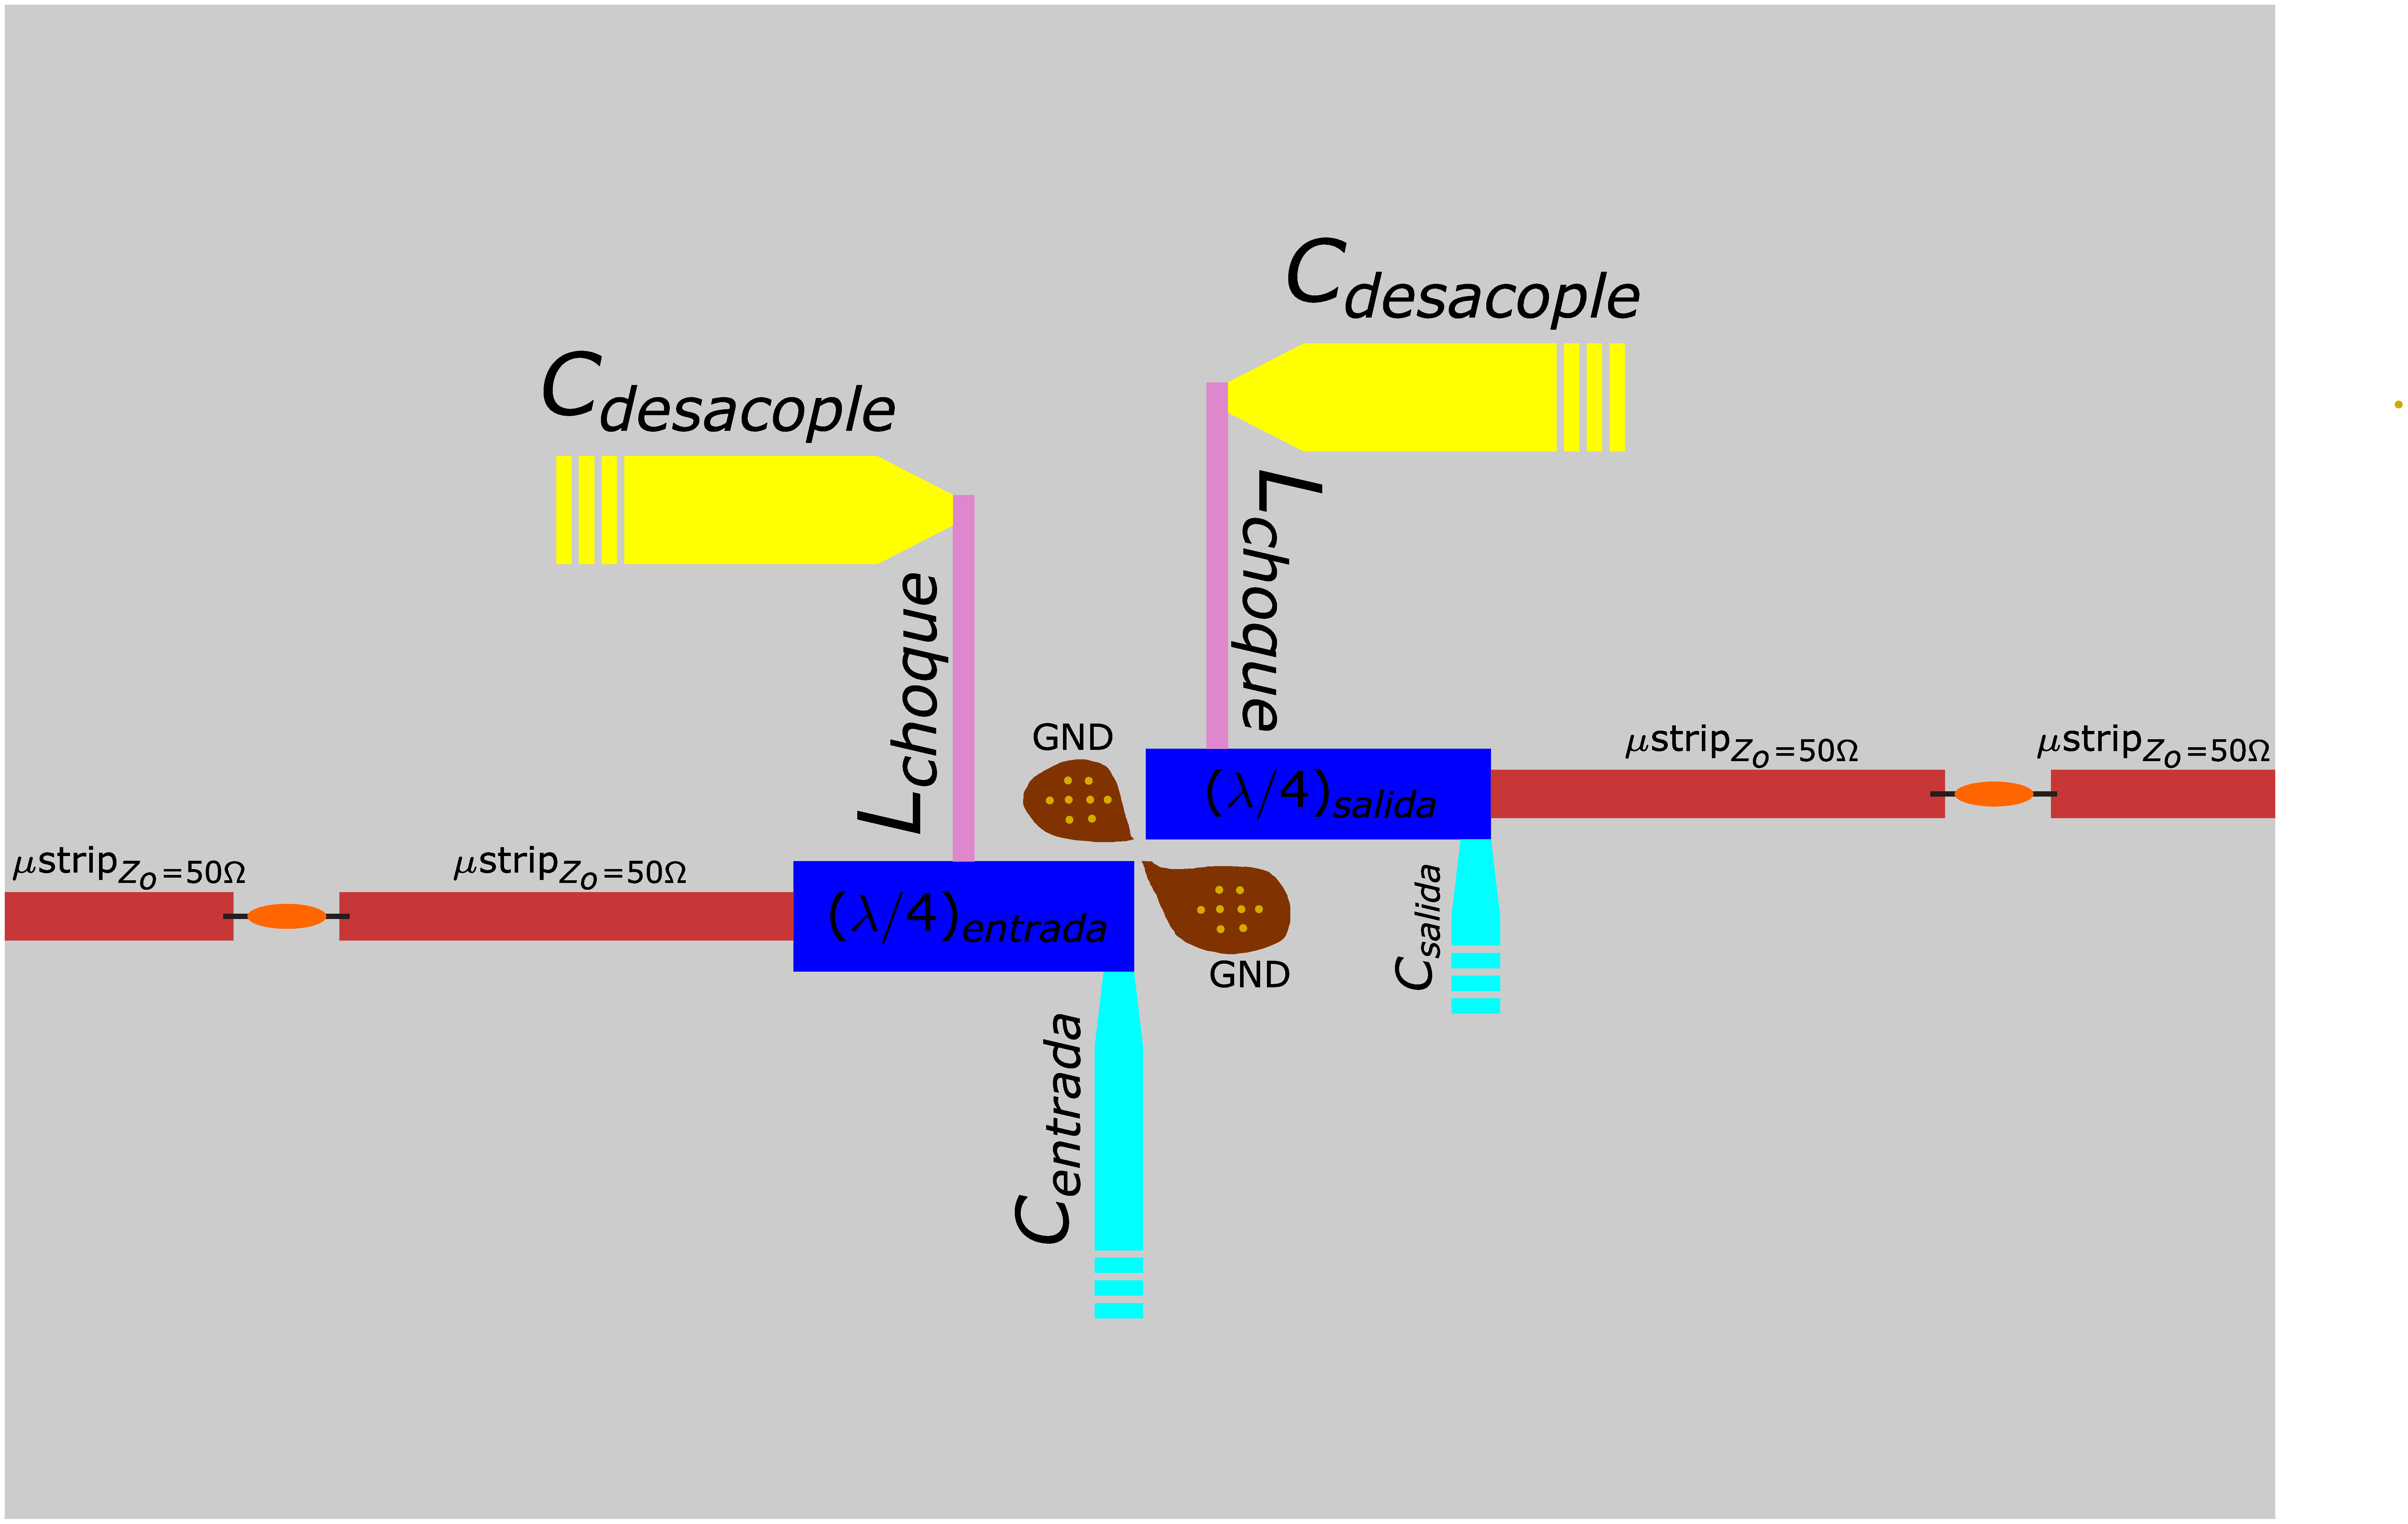
\includegraphics[width=0.8\linewidth]{img/layout}
			\caption{Layout implementado.}
			\label{fig:layout}
		\end{figure}
		
	\end{frame}
	
	\section{Simulación}
	
	\begin{frame}{Diseño en ADS}
		En el diseño del circuito, fue necesario implementar tapers, así como también gaps, de forma de aproximar más el circuito físico al ideal diseñado. Luego del añadido de los elementos mencionados, se corrió una instancia de optimización en el sistema, de forma de mejorar la respuesta en frecuencia de los parámetros de dispersión del circuito.
		
		De esto, se obtiene un circuito amplificador, que puede verse como una "caja negra", en donde los parámetros S ya no solo incluyen al transistor para una determinada polarización, sino que ya incluye el añadido de los diferentes parámetros de dispersión de las líneas de transmisión utilizadas.
	\end{frame}
	
	\begin{frame} {Resultados de la simulación (I)}
		El resultado de la simulación, en formato diagrama de Bode es el siguiente:
		\begin{figure}
			\centering
			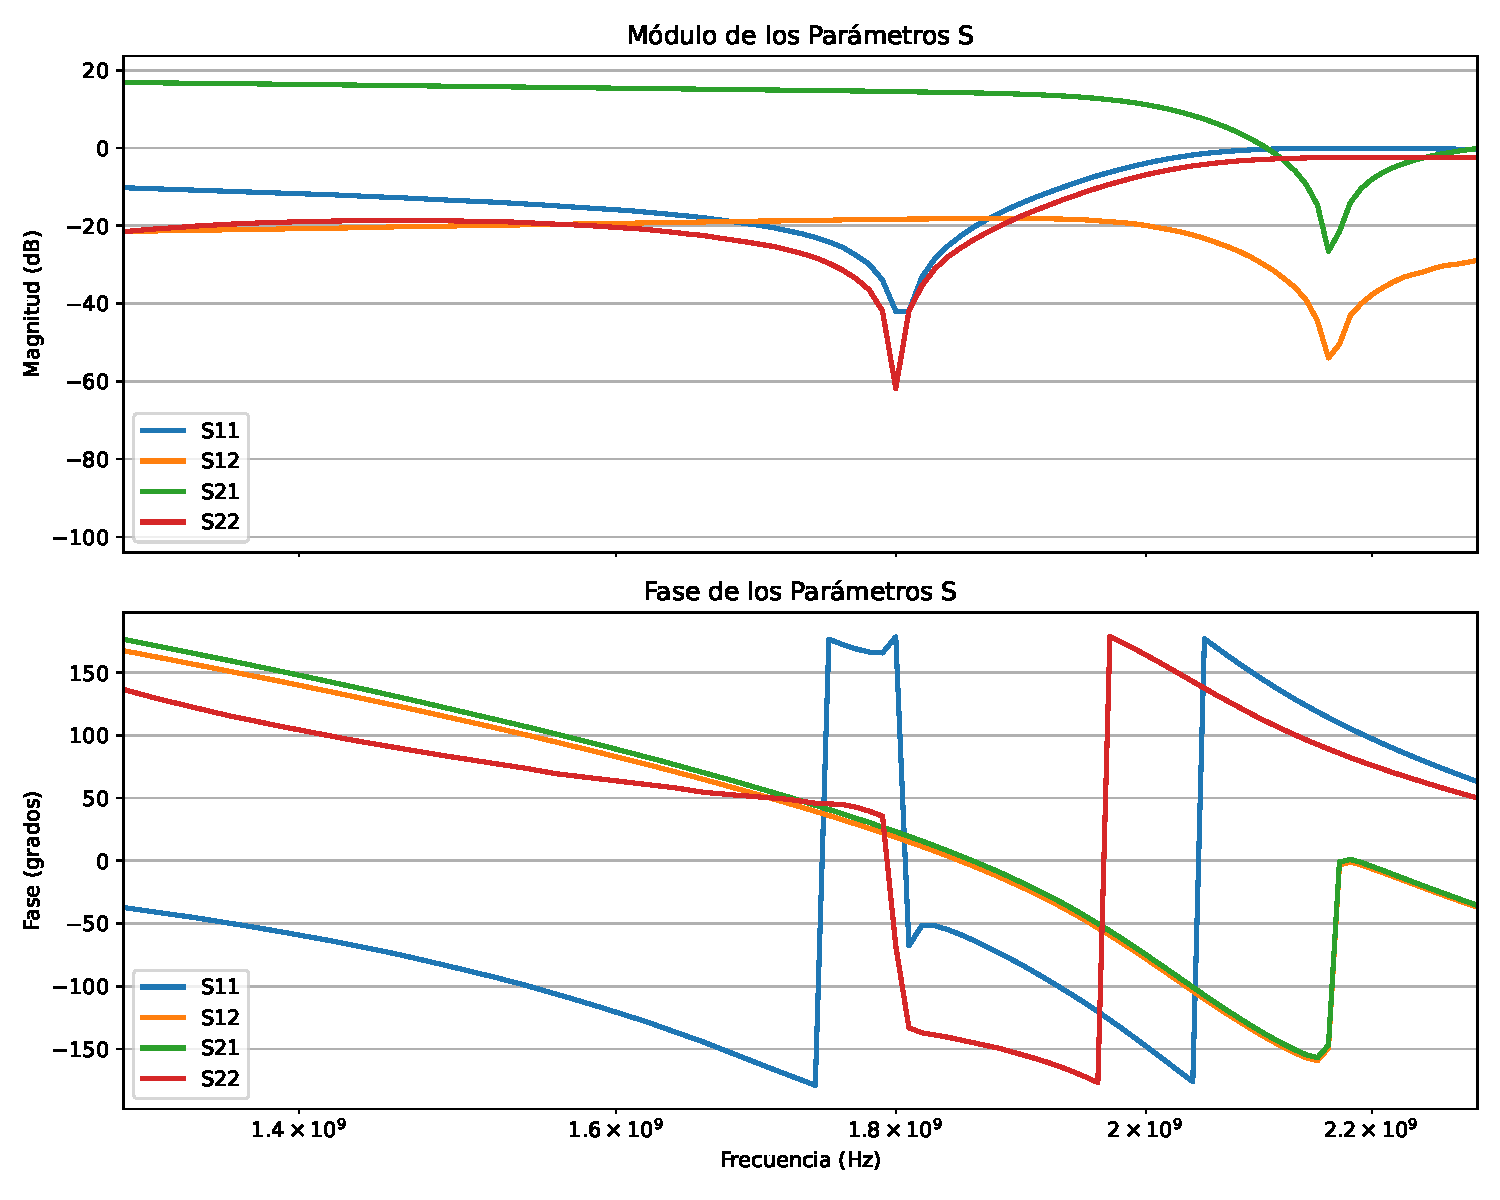
\includegraphics[width=0.7\linewidth]{../s_result}
			\caption{Resultado de la simulación de parámetros S.}
			\label{fig:sresult}
		\end{figure}
		
	\end{frame}
	
	\begin{frame}{Resultados de la simulación (II)}
		Ahora, los valores de interés son los siguientes:
		\begin{figure}
			\centering
			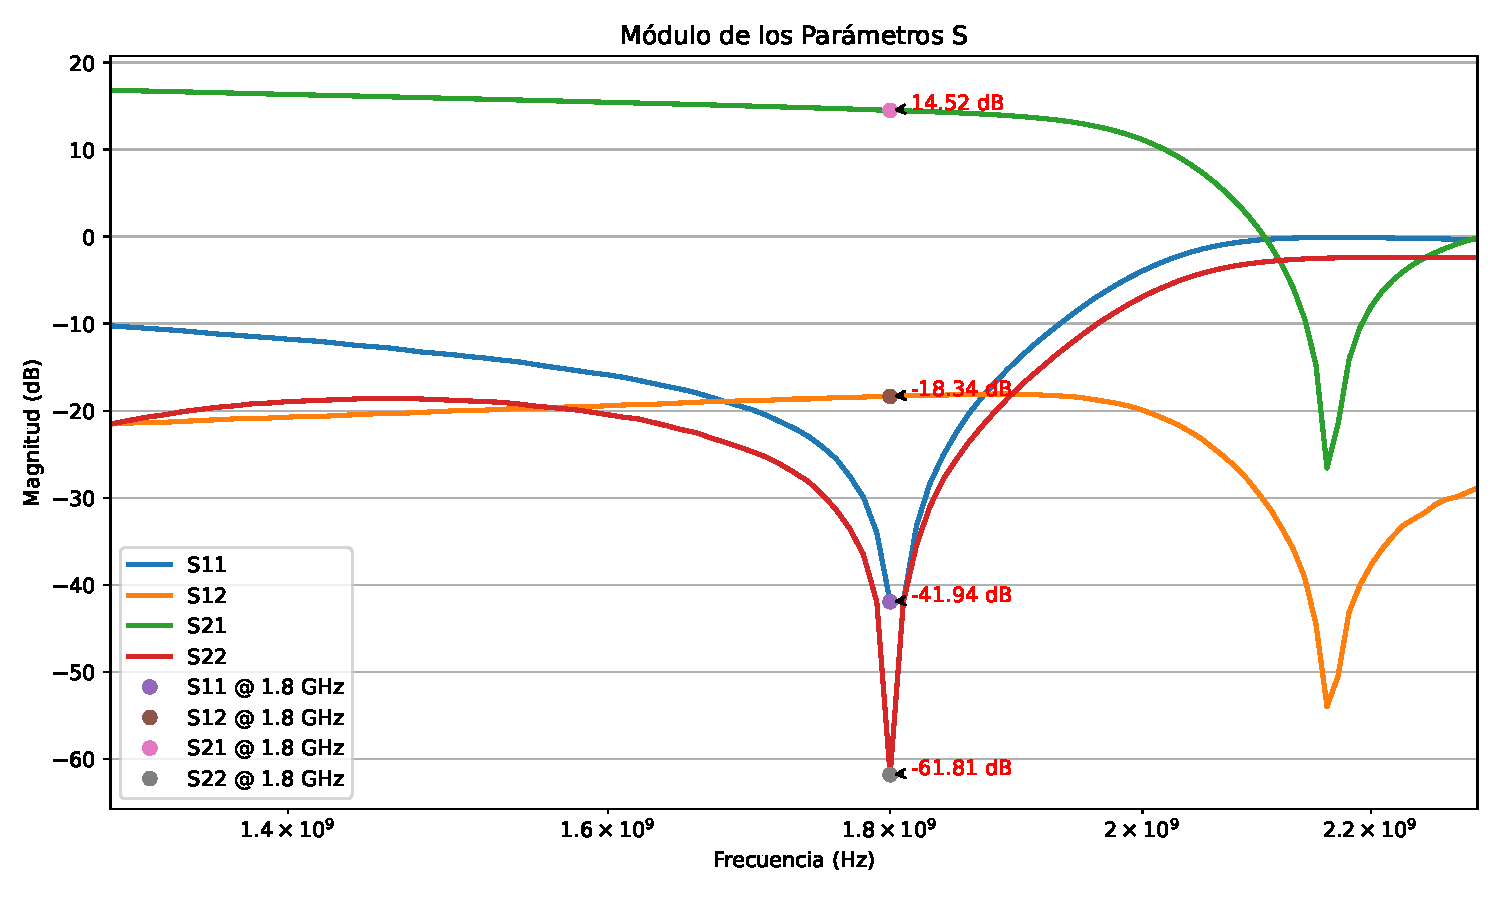
\includegraphics[width=0.7\linewidth]{../s_marker}
			\caption{Valores de interés para los parámetros S.}
			\label{fig:smarker}
		\end{figure}
		
	\end{frame}
	
	\begin{frame}{Resultados de la simulación (III)}
		El resultado de plotear los parámetros S obtenidos en la banda de frecuencias de $1.3$ a $2.3$ GHz en la carta de Smith de impedancias es el siguiente.
		\begin{figure}
			\centering
			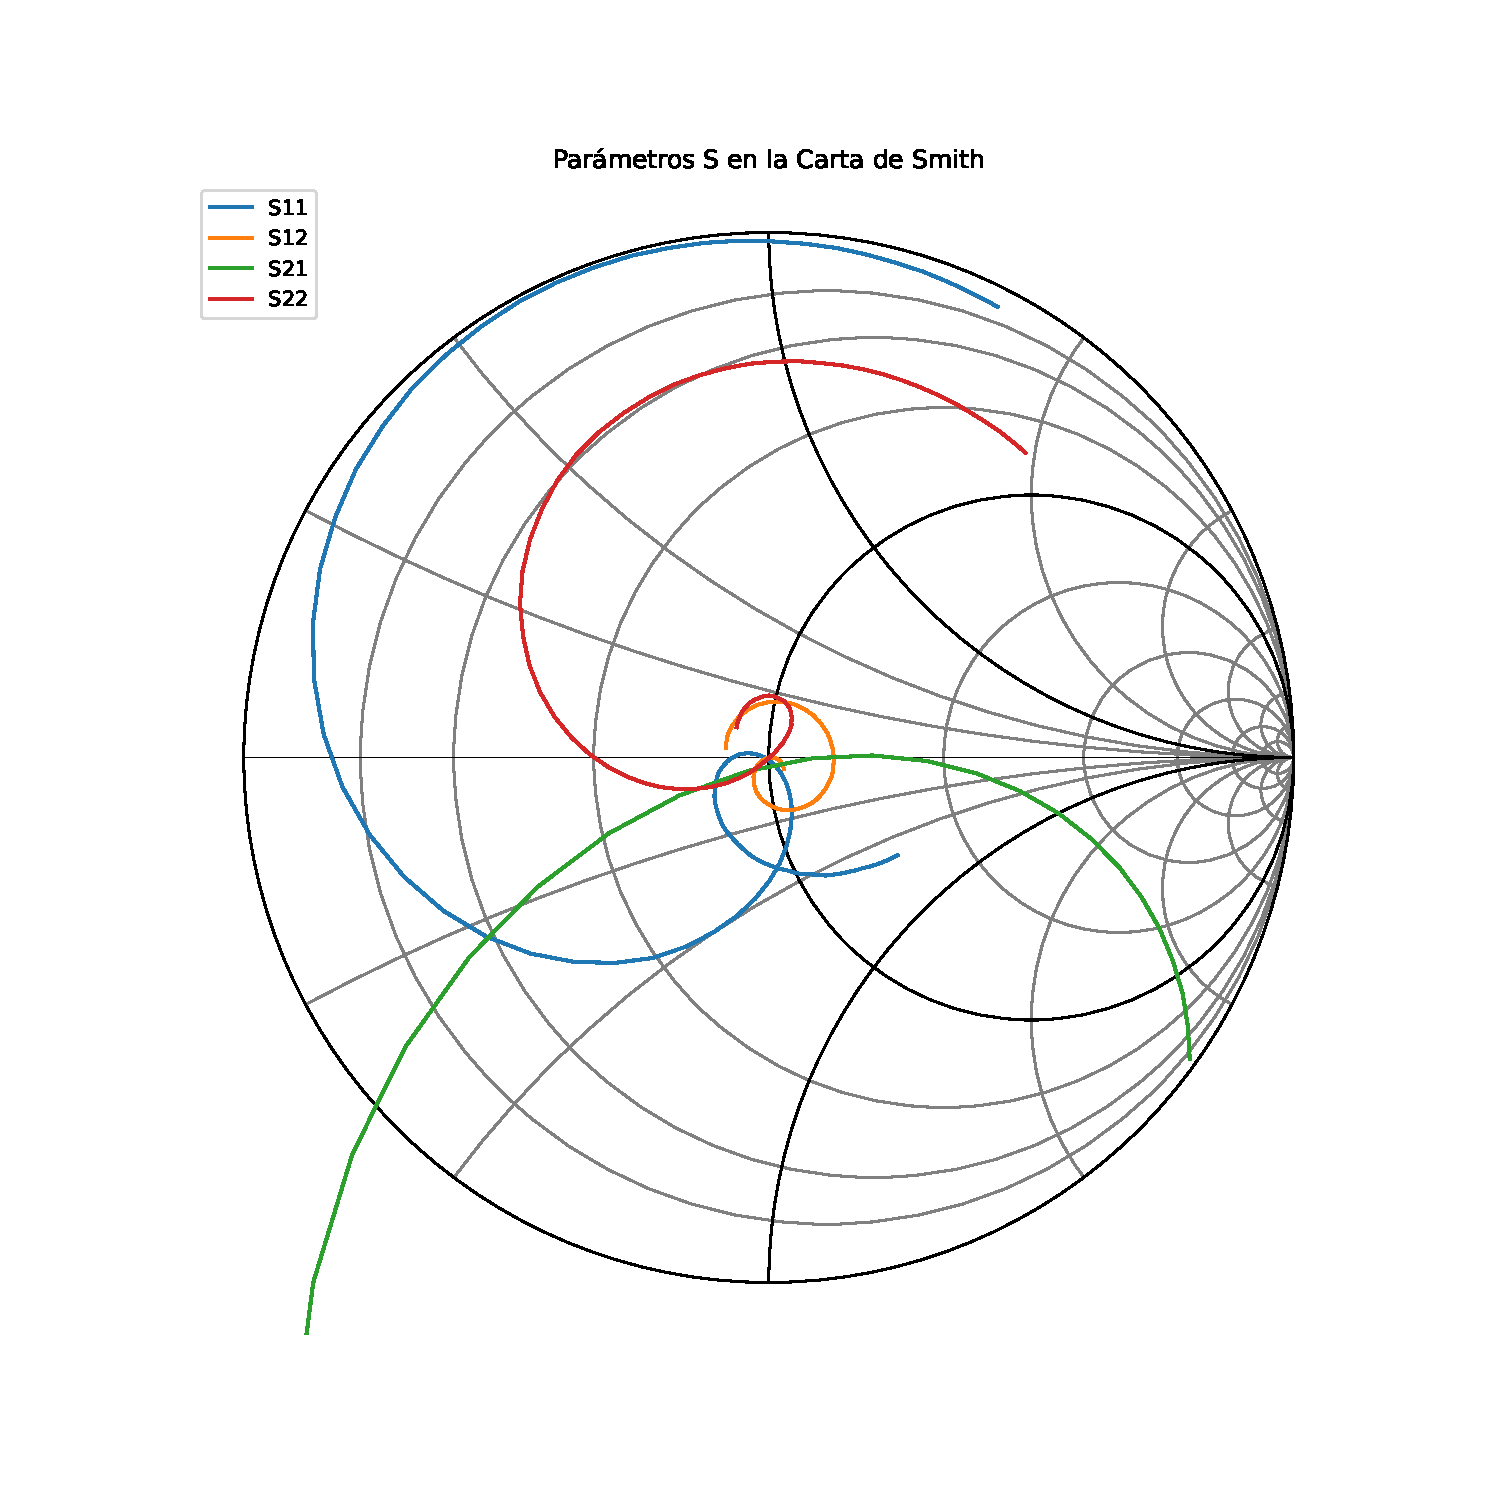
\includegraphics[width=0.5\linewidth]{../s_smith}
			\caption{Parámetros S en carta Smith.}
			\label{fig:ssmith}
		\end{figure}
		
	\end{frame}
	
	\section{Armado físico}
	
	\begin{frame}{Parte frontal}
		\begin{figure}
			\centering
			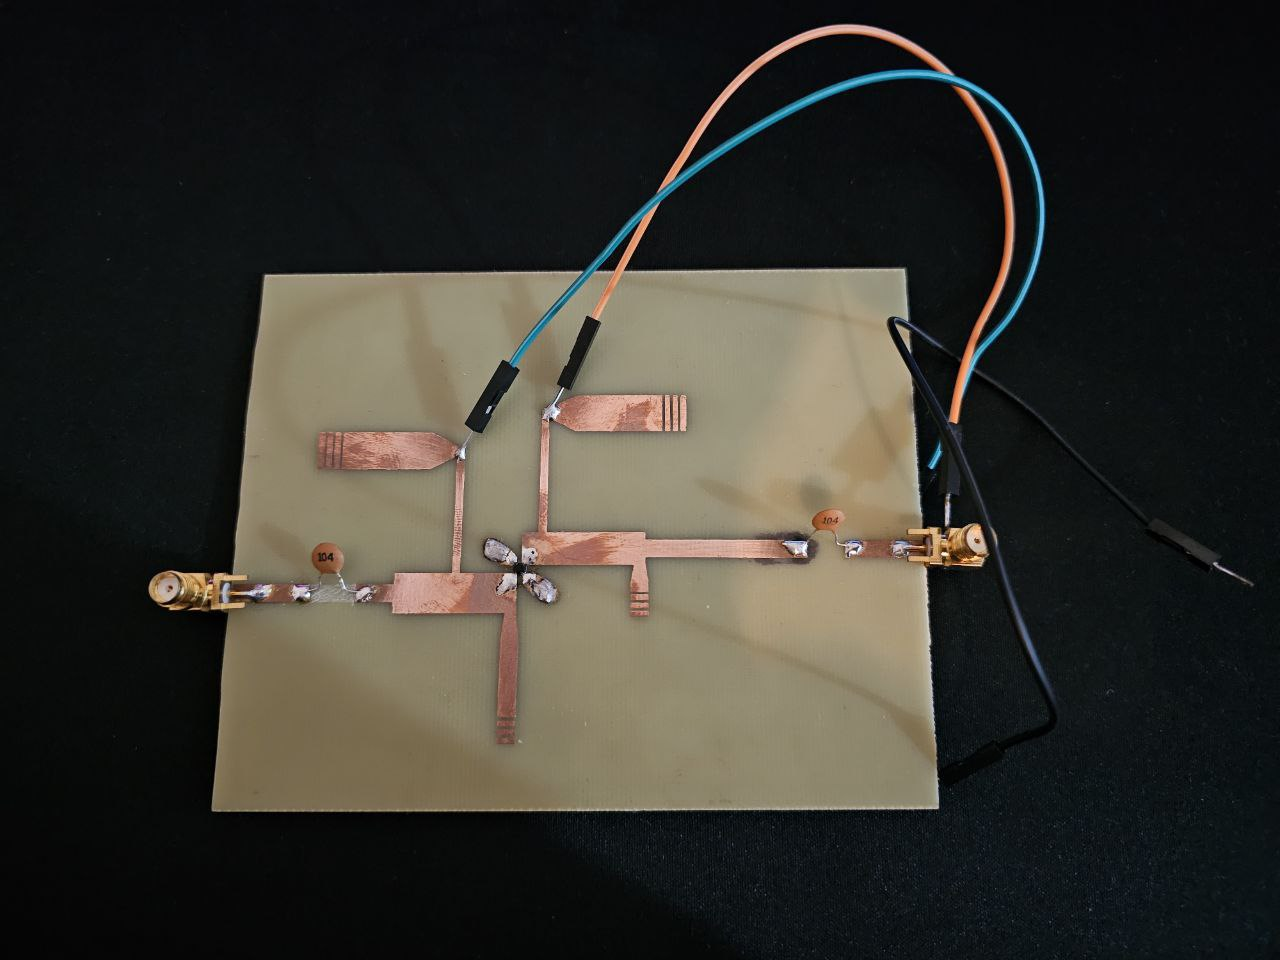
\includegraphics[width=0.7\linewidth]{../frente}
			\caption{Frente de la placa PCB.}
			\label{fig:frente}
		\end{figure}
	\end{frame}
	
	\begin{frame}{Plano de masa}
		\begin{figure}
			\centering
			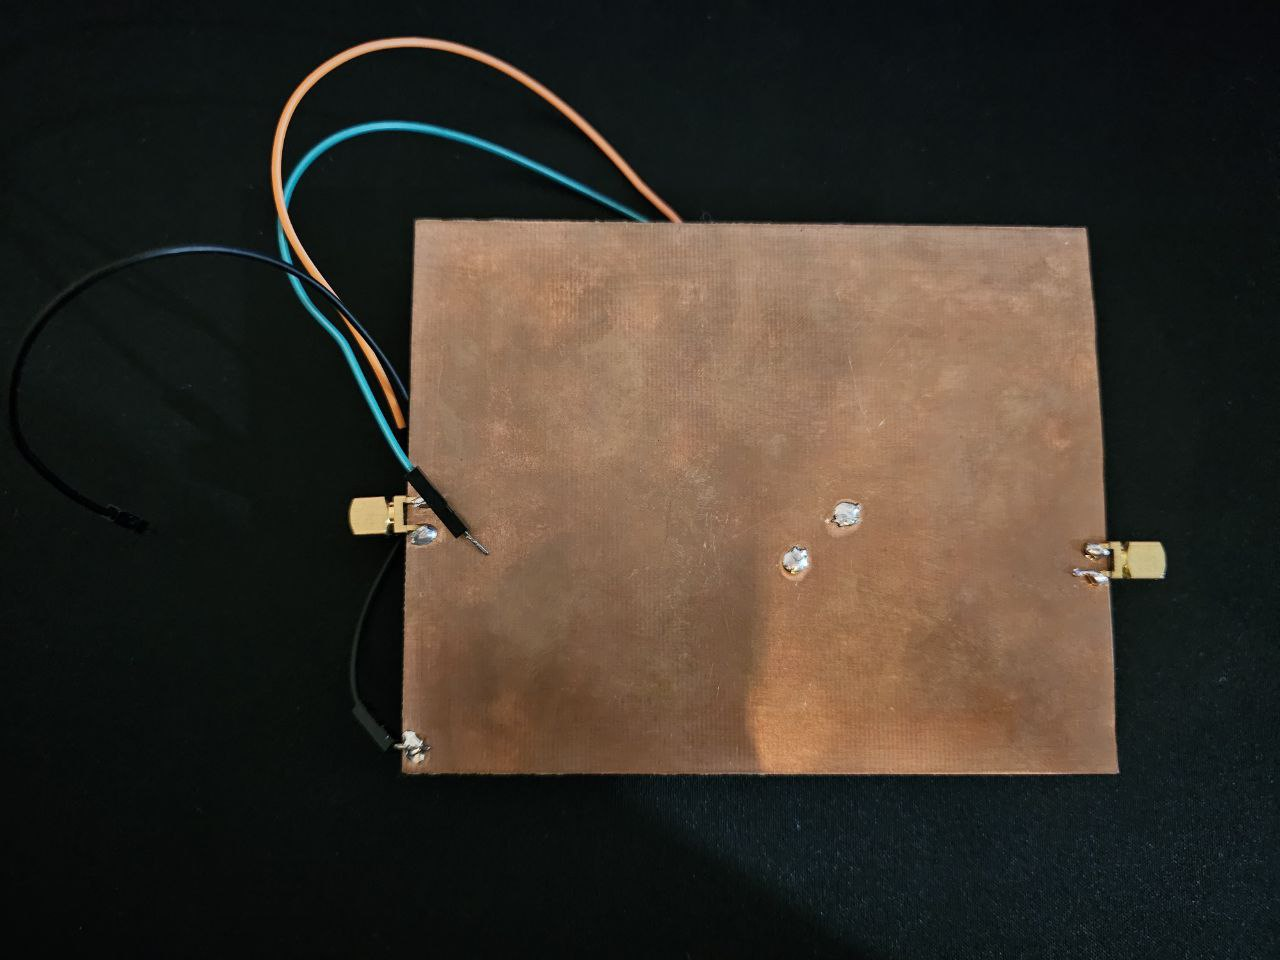
\includegraphics[width=0.7\linewidth]{../masa}
			\caption{Plano de masa de la placa PCB.}
			\label{fig:masa}
		\end{figure}
	\end{frame}
	
\end{document}